\hspace{-0.5mm}[13~v\textsuperscript{o}] si initio succedat exacte, erit medium punctum \textit{m}, sin rectifices solum usque ad \textit{r} et postea inverso tubo invenias \textit{s}, rursus rectificando ad medium differentiae inter \textit{r} et \textit{s}, et ita continuando, tertia aut quarta vice efficies, ut puncta \textit{m} et \textit{e} appareant in linea recta cum centro tubi duplicis. Hactenus de modo quo effici potest, ut diversa objecta utcunque integro semicirculo distantia simul videantur. \pend 
\count\Afootins=1200
\count\Bfootins=1200
\count\Cfootins=1200
\pstart \textso{Quarta pars} in qua quadrans noster excedit communis est exactitudo, qua altitudines sumi possunt, ope libellae aqueae \textit{water-level,}\edtext{}{\lemma{\textit{water-level,}}\Cfootnote{a.a.O., S. 61.}} ope cujus observator certus esse potest usque ad unum secundum aut duo. Ipsa libella est brevis tubus vitreus, longitudine 6 vel 8 pollicum, hermetice sigillatus utrobique, et repletus liquore qui neque congeletur, neque putrescat. Vitreus tubus sit quoad ejus fieri potest cylindricalis et rectus, quo propius recto, hoc exactius, dummodo habeat sensibilem curvaturam vel intumescentiam in medio; haec pars gibbosa erit superior, et tubus inclusus pyxidi cupreae\protect\index{Sachverzeichnis}{pyxis cuprea}. Vitrum \makebox[1.0\textwidth][s]{impleatur aqua distillata, cui circiter \rule[-2mm]{0pt}{9mm}$\displaystyle \frac{1}{3}$ bonae aquae fortis vel spiritus nitri affundatur,} 
\pend
\newpage
\pstart\noindent  ita neque putrescet, neque congelabitur. Fixetur in pyxide caemento duro. Et pyxis per cochleas firmabitur in latere quadrantis\protect\index{Sachverzeichnis}{quadrans} horizontali. 
\pend 
\pstart Brachio quadrantis\protect\index{Sachverzeichnis}{quadrans} immobili horizontaliter posito et limbo quadrantis\protect\index{Sachverzeichnis}{quadrans} sursum erecto, introspiciendo in centro observa dua objecta horizontalia, seu in horizonte posita, et sibi invicem opposita: observa limites bullae aereae in summitate liquoris in quolibet latere medii libellae, et fac notam, inde circumactis quadrantis\protect\index{Sachverzeichnis}{quadrans} extremis, pone donec extrema bullae stent ut in priore observatione inde rursus aspice eadem objecta in horizonte posita, et invenies differentiam inter priorem et hanc observationem; hanc biseca qua potes exactitudine, et aestimatione oculi pone dioptras\protect\index{Sachverzeichnis}{dioptra} in medio eorum inclinando quadrantem\protect\index{Sachverzeichnis}{quadrans}, inde per cochleam ita \edtext{rectifica libellam}{\lemma{rectifica}\Bfootnote{\textit{(1)}\ Tubum \textit{(2)}\ libellam, \textit{L}}}, ut extremum bullae aequaliter a medio distet, et rursus converte quadrantem\protect\index{Sachverzeichnis}{quadrans}, et vide an extremis bullae eodem loco stantibus duae oppositae dioptrae\protect\index{Sachverzeichnis}{dioptra} \edtext{telescopicae\protect\index{Sachverzeichnis}{telescopium} eadem objecta respiciant}{\lemma{telescopicae}\Bfootnote{\textit{(1)}\ videant \textit{(2)}\ eadem objecta respiciant; \textit{L}}}; quo posito certus eris perfectae horizontalitatis dioptrarum\protect\index{Sachverzeichnis}{dioptra} in fixo quadrantis\protect\index{Sachverzeichnis}{quadrans} brachio; sin minus tamdiu repetes examen donec succedat. Sed cum hoc genus perpendicularis subjectum sit incommoditati caloris et frigoris, quod rarefacit et condensat aeris bullam, et proinde facit bullam aeris minorem aut majorem; cura adhibenda est, ut varietates quae in ea producuntur per gradus caloris et frigoris, notentur. Quod ita facile efficies: Tubum ope glaciei et salis reduc ad quantum potes gradum frigoris; inde methodo proxime explicata, pone quadrantem\protect\index{Sachverzeichnis}{quadrans} horizontalem, et nota extrema bullae per 4.4. Inde paulatim aerem rarefac, et rursus observa expansionem et nota haec in vitro ope diamantis 3.3. vel 2.2. vel 1.1. vel 0.0. quo facto facillimum erit quovis tempore accommodare quadrantem\protect\index{Sachverzeichnis}{quadrans} ad exactitudinem desideratam cum appareant extensionis gradus; \textit{by being carefull to see, that the two ends of the bubble be proportionably extended, as to 00. 11. 22. 33. 44. etc. or to any intermediate space.}\edtext{}{\lemma{\textit{space}.}\Cfootnote{a.a.O., S. 62.}} Ratio exactitudinis haec est, quod superior pars \edtext{Tubi propinqua}{\lemma{Tubi}\Bfootnote{\textit{(1)}\ propior \textit{(2)}\ propinqua \textit{L}}} rectae lineae, ac proinde vel pars circuli ex ingenti radio vel quaedam curva irregularis circulo valde propinqua. Quantum ad hoc libellandi negotium, et ideo gradus \edtext{talis circuli proportionaliter}{\lemma{gradus}\Bfootnote{\textit{(1)}\ ejus pro \textit{(2)}\ talis circuli proportionaliter \textit{L}}} \edtext{erit magnus}{\lemma{erit}\Bfootnote{\textit{(1)}\ longus \textit{(2)}\ magnus, \textit{L}}}, et flexura tubi fieri potest ex curva radii tam magni, ut quaelibet secunda inclinationis producat in libella mutationem longitudinis valde sensibilis. Hoc difficulter efficietur communi via perpendiculorum seu plumborum suspensorum, nisi ex maxima pendeant altitudine, quod nec facile effici potest in praxi sine multa difficultate, et si obtineatur, nullius potest esse usus, ob magnitudinem apparatus, necessarii ad superan-
\pend
\newpage
\pstart\noindent dam structurae incertitudinem, et motum aeris, aliaque. Jam curvatura hujusmodi potest esse portio sphaerae radii 1000 pedum et ultra; et ideo minutum ejus non erit minus quam \rule[-5mm]{0pt}{12mm}$\displaystyle \frac{29}{100}$ pedis, et secundum minutum erit \textit{almost}\edtext{}{\lemma{\textit{almost}}\Cfootnote{a.a.O., S. 63.}} semicentesima pedis, quod sufficienter distingui potest nudo visu. Si cylinder vitreus sit 9 pollicum continebit duo minuta ejusmodi circuli, inter \textit{f} et \textit{f}. et unum inter 4 et 4. et ideo horizontalitas vitri hujus haberi potest ad certitudinem usque minuti secundi, quod vix alia ratione fieri potest. Sed restat difficultas ingens quomodo ejusmodi curvatura fieri possit, cum raro tubi vitrei reperiantur curvati, ut desiderari potest, et hoc tam est difficile quam invenire eos plane rectos. Hoc ut praeveniatur si adhibendae cannae vitreae, cura adhibenda, et varia tentamenta facienda, ut inveniatur quae vitra, et quae latera apta. Nam nostri vitri flatores non habent modum ea certo faciendi, curvaturae aut rectitudinis desideratae nec facile postea a tornatore eam accipiunt. Sed diligentia et tentamenta facile invenient ex multis in officina vitraria factis, aliqua. Ego uno usus sum alterius \edtext{formae \textit{25. fig., wich}}{\lemma{formae}\Bfootnote{\textbar\ \textit{25. fig.} \textit{erg.} \textbar\ , \textit{(1)}\ qui \textit{(2)}\ \textit{wich} \textit{L}}} \textit{i found to do, exceeding \edlabel{hooke3}well}\edtext{}{\lemma{\textit{well}}\Cfootnote{a.a.O., S. 64.}}\edtext{}{{\xxref{hooke3}{hooke4}}\lemma{\textit{well}}\Bfootnote{\textit{(1)}\ nigra parte aquam, lucida aerem repraesenta \textit{(2)}\ . Factus \textit{L}}}. Factus\edlabel{hooke4} erat is tubus ex duobus vitris \textit{drawn in distinct pipes at the glass-house but joyn'd together in the Lamp,}\edtext{}{\lemma{\textit{Lamp},}\Cfootnote{a.a.O., S. 64.}} et superior pars largioris vel inferioris Tubi, erat incurvata deorsum convexitate sua, ita ut aqua tangeret mediam partem, et bullae aeris extremo utriusque communicarent \edtext{invicem \textit{by the small pipe above}}{\lemma{invicem}\Bfootnote{\textit{(1)}\ per superiorem exiguam \textit{(2)}\ \textit{by the small pipe above.} \textit{L}}}\edtext{}{\lemma{\textit{above}.}\Cfootnote{a.a.O., S. 63.}}. Aliam etiam rationem expertus sum
%\begin{wrapfigure}{l}{0.4\textwidth}                    
%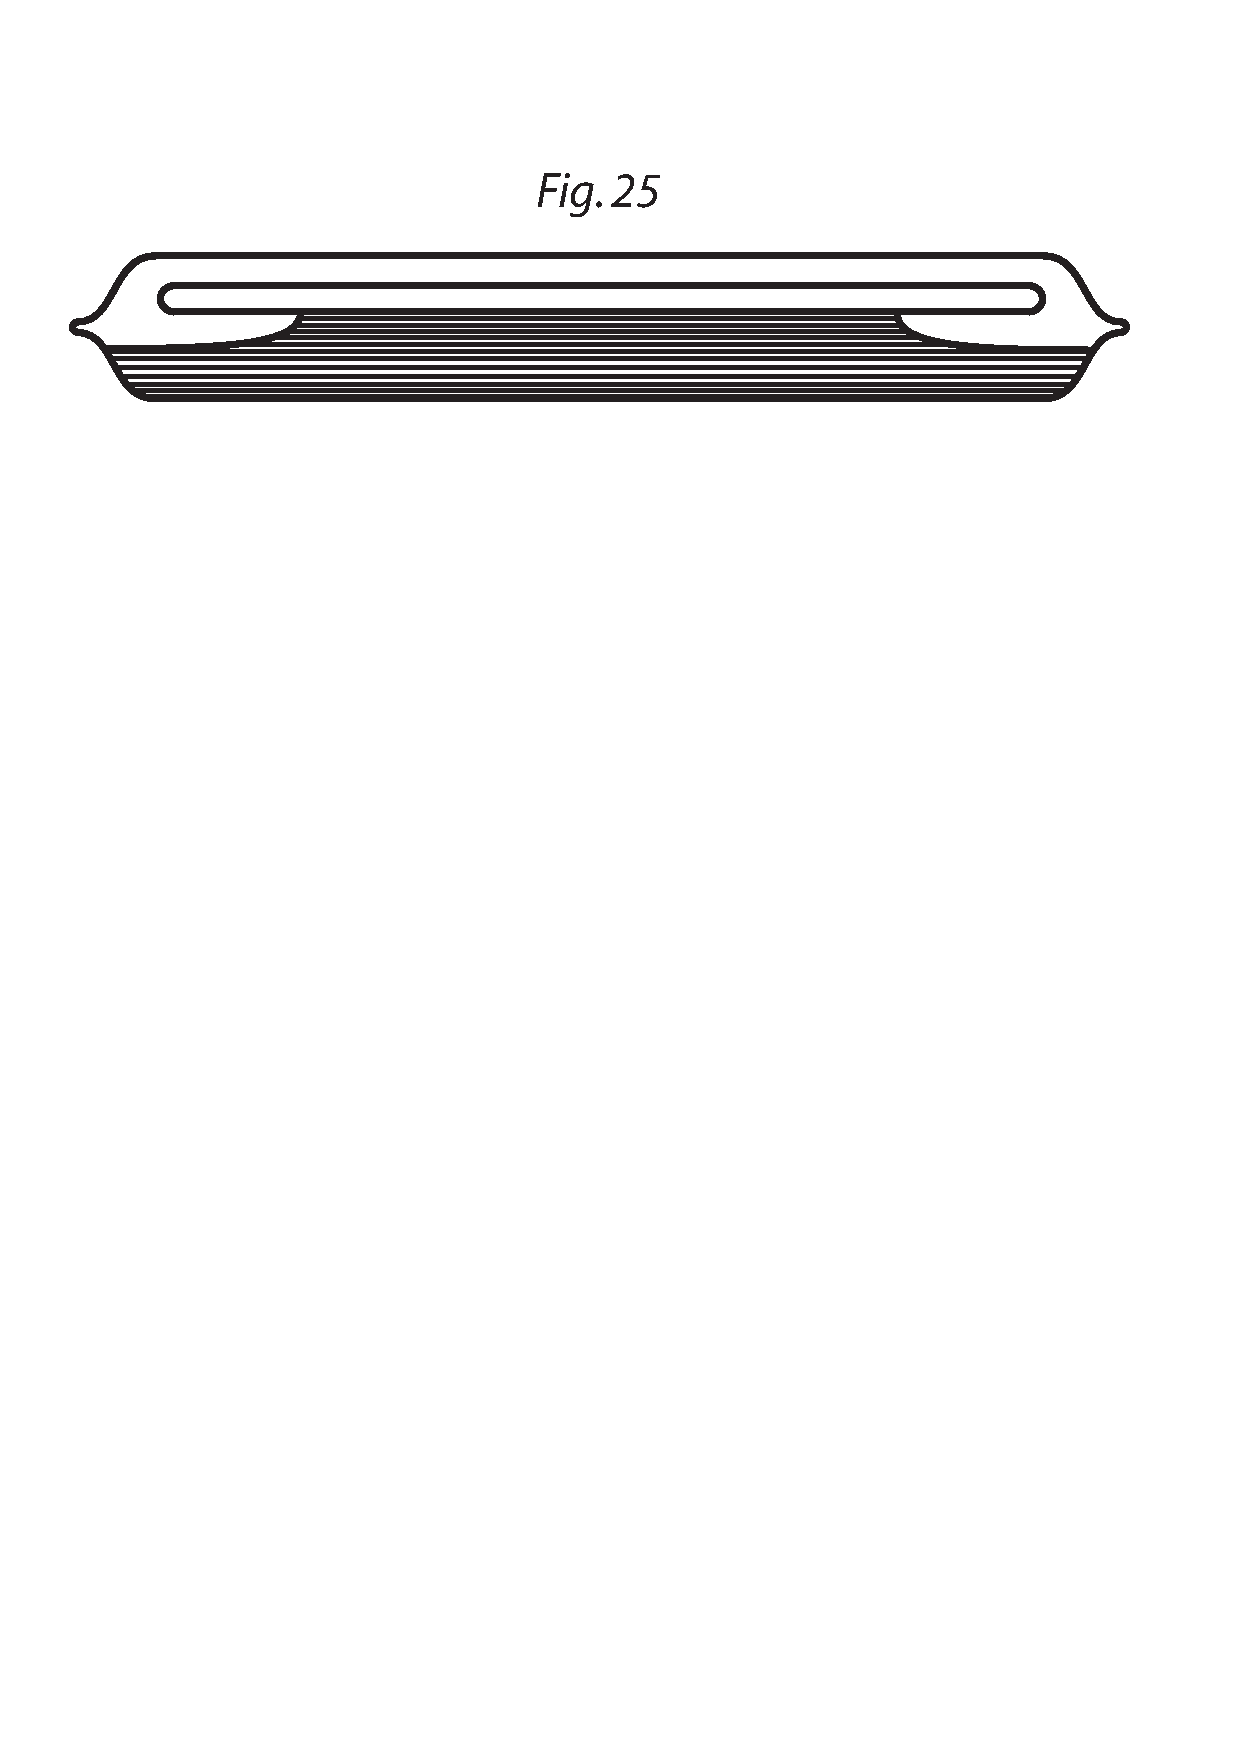
\includegraphics[width=0.4\textwidth]{images/LH0351506_013v-d1.pdf}\\
%\rule[0pt]{5mm}{0pt}[\textit{Fig. 6, nach Hooke Fig. 25}]
%\end{wrapfigure}
cujus ope certior fui curvitatis, et eam habui ex circulo majore. Hoc erat ope longi frusti speculi (\textit{looking glass plate}\edtext{}{\lemma{\textit{plate}}\Cfootnote{a.a.O., S. 64.}}) positi admodum quod ope [14~r\textsuperscript{o}]\edtext{}{\lemma{}\Afootnote{\textit{Oberhalb des Textes}: Pars III. Excerptorum ex Hookio contra Hevelium\vspace{-5mm}}} cochlearum\hfill tendebam\hfill (\textit{wich\hfill by\hfill the\hfill help\hfill of\hfill Screws\hfill i\hfill bent)\hfill upon\hfill the\hfill circular\hfill edges\hfill of\hfill a} 
\pend
%\vspace{0.5em}
\pstart
%\setline{26}
\noindent
\centering
%\begin{wrapfigure}{l}{0.4\textwidth}                    
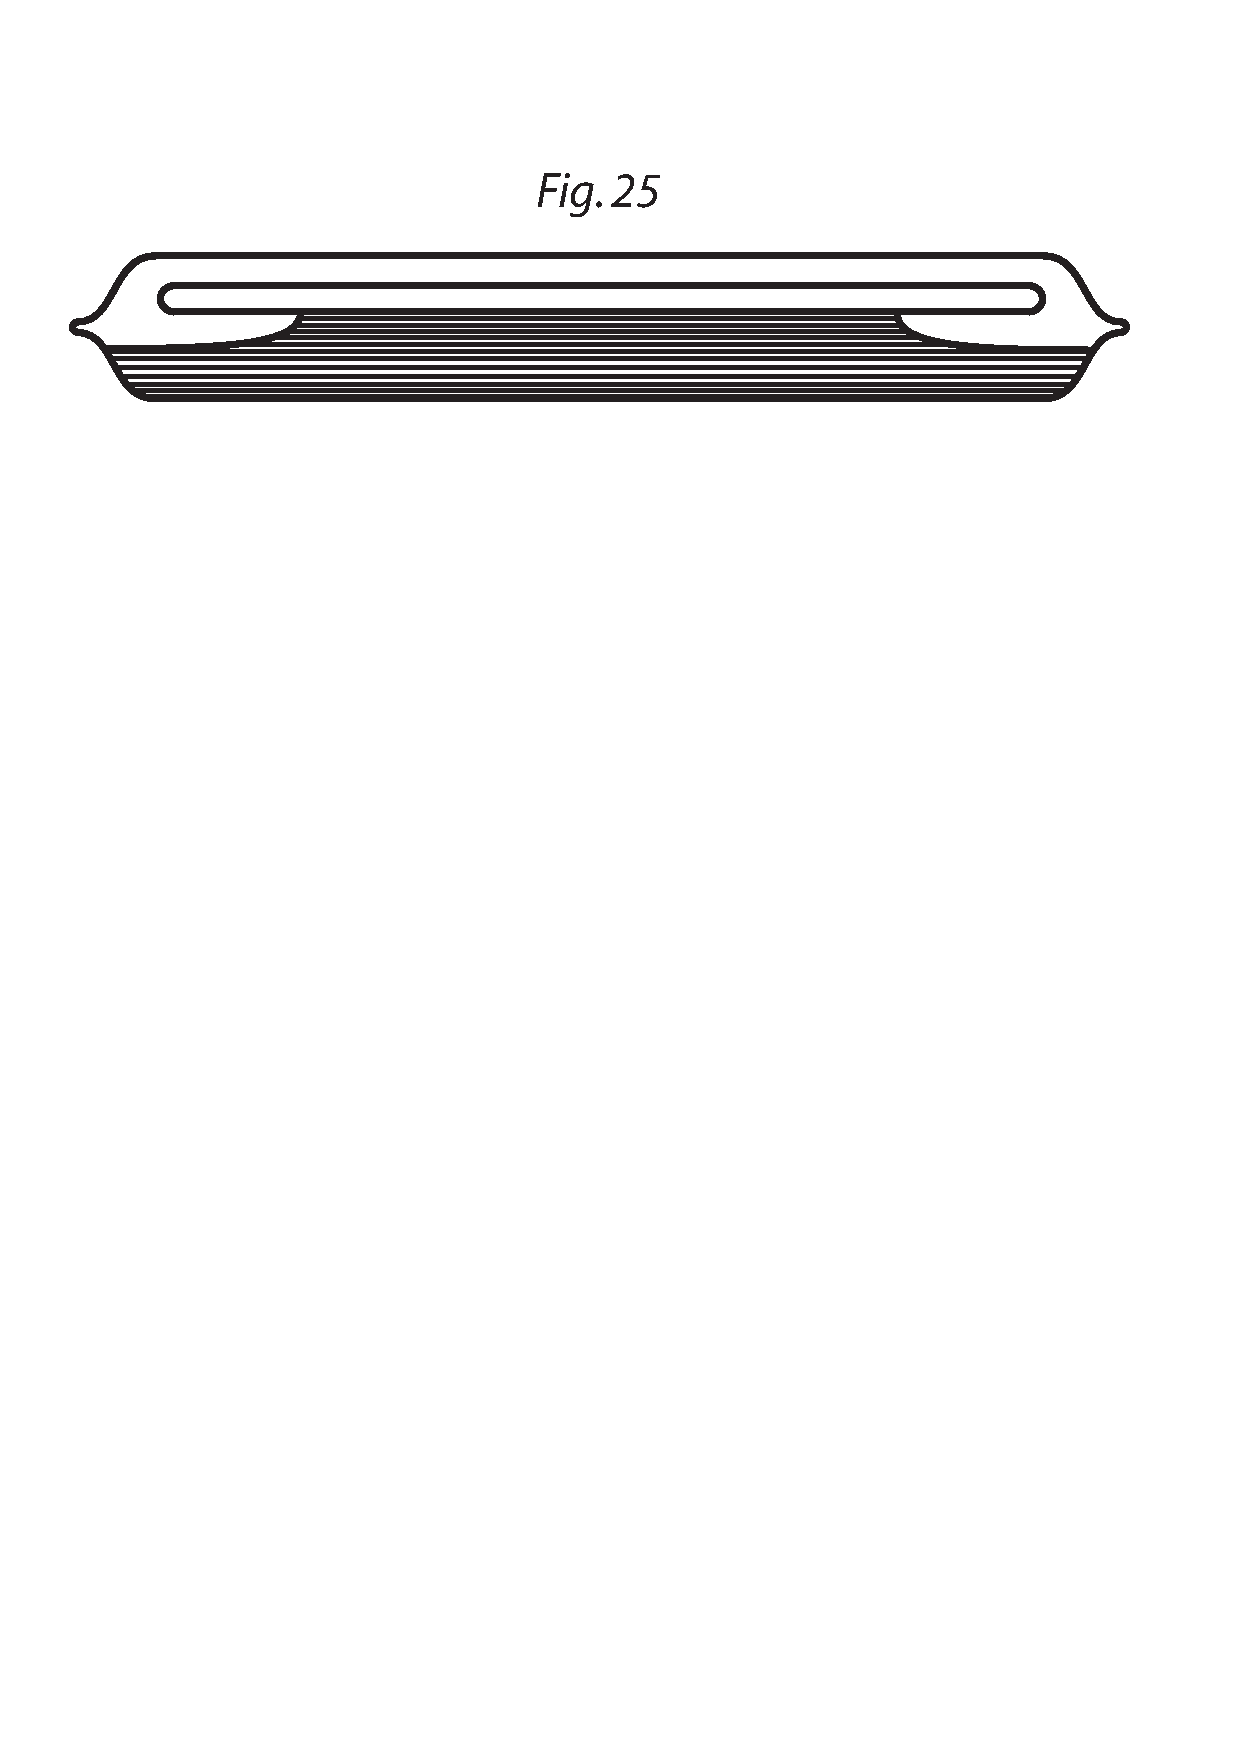
\includegraphics[width=0.6\textwidth]{images/LH0351506_013v-d1.pdf}\\
\centering \rule[0pt]{6mm}{0pt}[\textit{Fig. 6, nach Hooke Fig. 25}]
%\end{wrapfigure}
\pend 
\newpage
\pstart